\subsection{Functionality}%
\label{functionality-verif}
%
The end goal in this stage was to create a main system composed of subsystems
that interacted with protocols like Bluetooth, Wi-Fi, GPRS and RS232 to assure
the speed reference and wheel tilt commands reached the (virtual)
rover. Succeeding, the rover should move accordingly to those commands altering
its virtual coordinates.
After the phase of integrated testing, Section~\ref{sec:integrated-testing}, one can affirm that this goal was half met since the commands reach the virtual vehicle but only through one communication source (Bluetooth). The latter can also communicate back sending the alerts related to the status of the rover, once again resorting to Bluetooth. The final  
virtual environment block diagram is depicted in Fig.~\ref{fig:final-diagram}.
%
\begin{figure}[!ht]
\centering
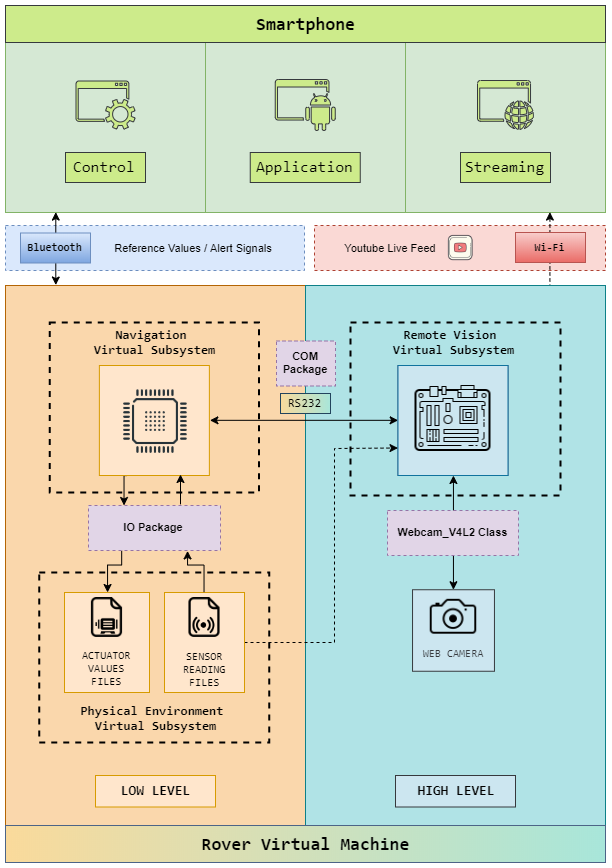
\includegraphics[width=0.85\textwidth]{img/functionality.png}
\caption{\label{fig:final-diagram}Final  
virtual environment block diagram view}
\end{figure}
%
\subsection{Communication}%
\label{comm-verif}
Considering subsystem communication the two parameters to verify were
Reliability and Redundancy, since the Communication Range was reliant on a physical prototype test.
%
\subsubsection{Reliability}%
\label{comm-verif-reliability}
Concerning Reliability, one needed to implement a system where the Wi-Fi dropped packets vs total packets ratio was monitored. However, since the system lacks the control message exchange through Wi-fi this goal is impossible to fulfil. Despite that, the Bluetooth control message exchange was implemented and tested.As these tests were made the package loss was analysed and one can conclude there is little to no package loss when sending the commands from the smartphone to the \gls{nvs} over Bluetooth since no message was lost. Despite not using a Wi-Fi, the Bluetooth protocol was still a reliable option.
%
\subsubsection{Redundancy}%
\label{comm-verif-redundancy}
Regarding redundancy, in the initial design (Fig.~\ref{fig:initial-design}) it was established the Wi-Fi as the main communication and the Bluetooth as redundancy communication. Later, the main communication was changed to Bluetooth and, as aforementioned, there is no redundancy communication for sending commands to rover when the latter fails.
%
%%% Local Variables:
%%% mode: latex
%%% TeX-master: "../../../dissertation"
%%% End:
